This tutorial will guide you through the basic features of StochSS. You will become familiar with the \textbf{Model Editor} and with the \textbf{Simulation Manager}. You will learn how to create your own model, which can be population or concentration-based, and how to simulate it, locally or in the cloud, using either an ordinary differential equation (ODE) solver or the stochastic simulation algorithm (SSA).

\section{\label{sec:acc} Creating Administrator and Standard User Accounts}
At the end of a successful installation process, your default browser will launch, and you will be asked to create an admin account as in Figure \ref{fig:admin} (the is only one admin account for the entire system).
Once the admin account is created you will be forwarded to a regular login page (Figure \ref{fig:login}) where the admin and the approved users can log in to a StochSS server.

\begin{figure}[!htb]
\centering
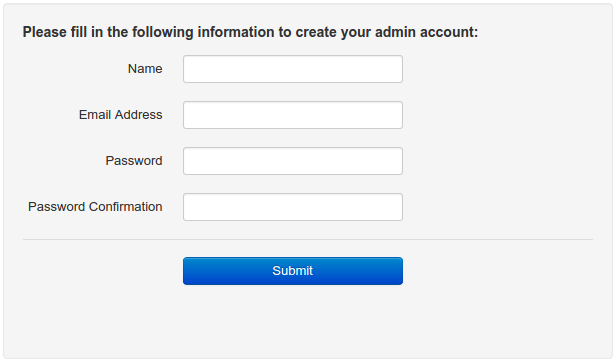
\includegraphics[scale=0.64]{T1/admin.png}
\caption{Administrator login page}
\label{fig:admin}
\end{figure}

Users can click \textbf{Create Account} to request an account.
The account will not be accessible until the admin approves it in the \textbf{Admin Panel} (the admin can also delete active users as well as reset their passwords there).

\begin{figure}[!htb]
\centering
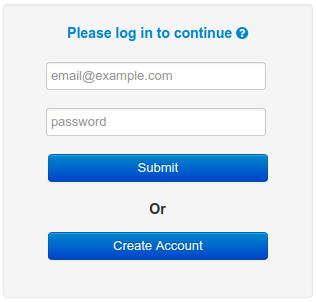
\includegraphics[scale=0.64]{T1/login.png}
\caption{User login page}
\label{fig:login}
\end{figure}

\section{\label{sec:imp} Importing a Model}
The \textbf{Model Editor} will let you create new or modify existing well-mixed stochastic biochemical models as well as deterministic models based on ODEs.
The best way to get started with the model editor is to import an example model and look at the different sections.

\subsection{Importing an existing model}

\underline{Option 1: StochSS Public Library}
\begin{itemize}
  \item Navigate to the main \textbf{Model Editor} page.
  \item Click the \textbf{Import from Public Library} link in the right-hand toolbar.
  \item Select a model (birthdeath is simple) from the Public Library and click \textbf{Copy Model to Library}.
\end{itemize}

\underline{Option 2: Stochkit2 .XML}
\begin{itemize}
  \item Navigate to the main \textbf{Model Editor} page.
  \item Click the \textbf{Import from .XML} link in the right-hand toolbar.
  \item Select an XML file. A collection of example models can be found in the \textbf{examples} directory within the StochSS install folder (examples/birthdeath.xml is simple).
  \item Click on the \textbf{Import} button.
\end{itemize}

After importing the XML file or public model StochSS should display the imported model in the model editor.
Take a look through the page at how the different \textbf{Species}, \textbf{Parameters} and \textbf{Reactions} are defined.
By clicking \textbf{Export to .zip} or \textbf{Export to Public Library} the model can be shared across computers (using \textbf{Import from .zip}) or shared amongst users of the same StochSS.

\section{Creating a New Model}
An example population model is defined by the following two reactions:
\[ \begin{cases}
S0 + S0 \xlongrightarrow{k1} S1 \nonumber \\
S1 \xrightarrow{k0} \emptyset . \nonumber 
\end{cases} \]

To create this model in the \textbf{Model Editor}:
\begin{itemize}
  \item Navigate to the \textbf{Model Editor}.
  \item Click \textbf{Add Model} and select \textbf{Population, Well-mixed}.
  \item Rename the model \textbf{example}.
  \item Click the \textbf{Create Species} button twice to create two species.
  \item By default, they are named \textbf{S0} and \textbf{S1}. Set the initial condition for \textbf{S0} to \textbf{1000} and the initial condition for \textbf{S1} to \textbf{0}.
  \item Similarly to above, click \textbf{Add Parameter} twice to add two parameters.
  \item By default they will be named \textbf{k0} and \textbf{k1}. Set \textbf{k0} to \textbf{0.0001} and \textbf{k1} to \textbf{0.05}.
  \item Use the \textbf{Add Reaction} button to add the two reactions above. Select the reactants, products, rates and reaction types corresponding to the equations above. Use Figure \ref{fig:reaction1} and \ref{fig:reaction2} to verify the settings.
\end{itemize}

\begin{figure}[!htb]
\centering
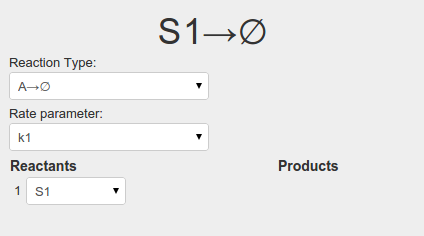
\includegraphics[scale=0.64]{T1/reaction1.pdf}
\caption{Dimerization reaction}
\label{fig:reaction1}
\end{figure}

\begin{figure}[!htb]
\centering
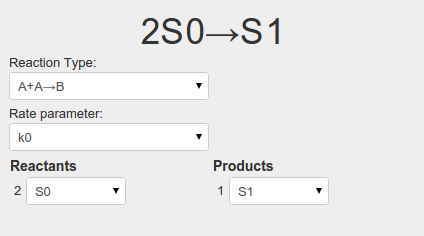
\includegraphics[scale=0.64]{T1/reaction2.pdf}
\caption{Decay reaction}
\label{fig:reaction2}
\end{figure}

\section{Running a Simulation and Visualizing results}

For this section, create or import a model using the directions above.

\begin{itemize}
  \item Navigate to the \textbf{Simulation Manager} page.
  \item Select the model you wish to simulate and click on the \textbf{Next} button.
  \item Setup your simulation parameters: name, time, data storage frequency, realizations and solver type. 
  \begin{itemize}
    \item If you are simulating a population-based model you can choose between the deterministic and the stochastic solvers.
    \item If you choose the deterministic solver, you have the possibility to perform sensitivity analysis on a set of chosen parameters related to your model.
    \item Concentration-based models can only be simulated using the deterministic solver.
  \end{itemize}  
  \item Click on the \textbf{Run Locally}. When the job runs, StochSS should automatically transition to the \textbf{Job Status} page
  \item Click the \textbf{View} link beside the recently run job to open the \textbf{Job summary} page where you can plot the simulation's trajectories.
  \item Clicking \textbf{Access Local Data} downloads a raw copy of the data. This can be used to shared data between StochSS installations or accessed manually if necessary.
\end{itemize}

\subsection{Converting a concentration model to population}
Create a concentration model or use the directions above to import one. Both Lotka-Volterra examples are concentration models (and are available both as .XMLs and Public Library models).

\begin{itemize}
  \item Select the newly minted concentration model.
  \item Click on \textbf{Convert to Population} item on the right-hand toolbar to start the conversion process. The model conversion page will open.
  \item To convert a concentration model to a population, a system volume must be specified. This can be done at the bottom of the page.
  \item Given a volume, StochSS will convert the species initial conditions (simply $initial\_condition\_population = initial\_condition\_concentration * volume$) and \textbf{attempt} to convert the reaction rates. It is not always possible to convert reaction rates automatically. In the case automatic conversion fails, the conversion can still proceed but the user is expected to fix whichever reaction could not be converted automatically.
  \item Click the \textbf{Finish conversion} button at the bottom right of the page to create a population-based model. This newly created population model can be simulated using both deterministic and stochastic solvers.
  \item Click \textbf{Cancel conversion} to cancel the conversion.
\end{itemize}

\warning{The conversion process operates correctly only if the model to be converted is entirely based on the mass action kinetics allowed in Gillespie Stochastic Simulation Algorithm \cite{dan}. If the model to be converted is not entirely based on mass action kinetics, the conversion tool only converts what it can. }

\section{Backup and Transfer your Data}
You can backup or share your saved models and simulations with the StochSS .zip format. There three ways to create StochSS .zips:

\begin{itemize}
\item Navigating to the \textbf{Backup} page in the left-hand toolbar and clicking \textbf{Export}. This exports a .zip containing all models and simulation results for the current user. There is an option to export all data for all users if this page is accessed with the admin account.
\item Selecting a model in the \textbf{Model Editor} page and clicking \textbf{Export to .zip}.
\item Clicking the \textbf{View} link to view a job's results and then clicking \textbf{Access local data}.
\end{itemize}

These .zip files can all be imported into StochSS in the \textbf{Backup} page. To import the contents of a .zip file into StochSS:

\begin{itemize}
\item Navigate to the \textbf{Backup} page.
\item Click the \textbf{Import} tab.
\item Select the .zip file to upload. The file should automatically begin uploading, and then appear in a table of .zip archives below.
\item Define the behaviour of the import by either limiting what files get imported, or how overlapping names are handled.
\item Click the \textbf{Import} button at the bottom of the page.
\end{itemize}

\subsection{Exporting data from an old StochSS (<= StochSS 1.2)}
To create a backup archive from an older version of StochSS execute the following command from a terminal window in the directory of your new StochSS installation:
\begin{verbatim}
./exportserver.py path_to_your_old_StochSS_installation
\end{verbatim}
You can import a backup archive you created with an older version of StochSS as described above.

